% "Hidden in the Leftovers": course project proposal (CL3.412). Build: latexmk -xelatex proposal.tex
% Pages 1-3 are the proposal; the appendices hold the original plan and every detail of the pilot study.
% Numbers come from docs/handoff/data/*.csv and the main pilot run results/paper_20261026_001341 (metrics, DECISIONS.md,
% SUMMARY.md), the quick pilot results/pilot_20261025_230749, results/task_analysis and results/check_forward.
% Figures: figures/p_*.pdf (scripts/make_proposal_figures.py); diagrams: diagrams/*.tex (TikZ).
\documentclass[11pt,a4paper]{article}

\usepackage{amsmath}
\usepackage{fontspec}
\usepackage[a4paper,margin=2cm,top=1.9cm,bottom=1.8cm,headsep=0.45cm]{geometry}
\usepackage{graphicx}
\usepackage{booktabs}
\usepackage{tabularx}
\usepackage{array}
\usepackage{xcolor}
\usepackage{enumitem}
\usepackage[font=small,labelfont={bf,color=accent},skip=4pt]{caption}
\usepackage{float}
\usepackage{placeins}
\usepackage{fancyhdr}
\usepackage{tikz}
\usetikzlibrary{arrows.meta,positioning,calc,decorations.pathreplacing}
\usepackage[numbers,sort&compress]{natbib}
\usepackage{hyperref}

\definecolor{accent}{HTML}{2a78d6}
\definecolor{muted}{HTML}{8a8985}
\definecolor{light}{HTML}{c9c7c1}
\definecolor{ink2}{HTML}{5f5d58}
\definecolor{paper}{HTML}{f6f5f2}
\colorlet{linkblue}{accent!75!black}
\hypersetup{colorlinks=true, linkcolor=linkblue, citecolor=linkblue, urlcolor=linkblue,
  pdftitle={Hidden in the Leftovers}, pdfauthor={Prakhar Singhal, Raveesh Vyas}}
\graphicspath{{figures/}}

% Hindi examples: Devanagari if a font with the script is installed (serif preferred, to match the body text),
% else a transliteration.
\IfFontExistsTF{Noto Serif Devanagari}{%
  \newfontfamily\devanagarifont[Script=Devanagari,Scale=0.95]{Noto Serif Devanagari}%
  \newcommand{\hindi}[2]{{\devanagarifont #1}}%
}{\IfFontExistsTF{Noto Sans Devanagari}{%
  \newfontfamily\devanagarifont[Script=Devanagari,Scale=0.92]{Noto Sans Devanagari}%
  \newcommand{\hindi}[2]{{\devanagarifont #1}}%
}{%
  \newcommand{\hindi}[2]{\textit{#2}}%
}}
\newcommand{\lat}[1]{{\normalfont #1}} % Latin letters and digits inside Devanagari text

\setlist{nosep,leftmargin=1.4em}
\setlength{\parskip}{3pt}
\setlength{\parindent}{0pt}
\setlength{\textfloatsep}{10pt}
\setlength{\intextsep}{8pt}
\renewcommand{\arraystretch}{1.12}
\newcolumntype{Y}{>{\raggedright\arraybackslash}X}
\newcommand{\prompt}[1]{\texttt{\small #1}}
\newcommand{\term}[1]{\textbf{#1}}
\captionsetup[table]{position=top}

% Page furniture: a small running head and the page number.
\pagestyle{fancy}
\fancyhf{}
\fancyhead[L]{\footnotesize\color{muted}Hidden in the Leftovers}
\fancyhead[R]{\footnotesize\color{muted}CL3.412 course project proposal \textperiodcentered\ Team IpCp-{}-}
\fancyfoot[C]{\footnotesize\color{muted}\thepage}
\renewcommand{\headrulewidth}{0.4pt}
\renewcommand{\headrule}{{\color{light}\hrule height\headrulewidth}}
\fancypagestyle{plain}{\fancyhf{}\fancyfoot[C]{\footnotesize\color{muted}\thepage}\renewcommand{\headrulewidth}{0pt}}

\makeatletter
\renewcommand\section{\@startsection{section}{1}{\z@}{-1.6ex plus -.4ex}{0.6ex}{\large\bfseries\color{accent}}}
\renewcommand\subsection{\@startsection{subsection}{2}{\z@}{-1.2ex plus -.3ex}{0.4ex}{\normalsize\bfseries}}
\renewcommand\maketitle{\thispagestyle{plain}{\centering
  {\LARGE\bfseries \@title\par}\vspace{3pt}
  {\large Task-Specific Reconstruction Gaps of Sparse Autoencoders\\in English and Indian Languages\par}\vspace{6pt}
  {\@author\par}\vspace{3pt}
  {\color{muted}\small Mechanistic Interpretability of Language Models (CL3.412)\\
    Course project proposal\;\textperiodcentered\; Team IpCp-{}-\;\textperiodcentered\; \@date\par}}
  \vspace{6pt}}
\makeatother

% The short summary box.
\newcommand{\inshort}[1]{\par\noindent\colorbox{paper}{\parbox{\dimexpr\linewidth-2\fboxsep}{\vspace{3pt}#1\vspace{3pt}}}\par}

\title{Hidden in the Leftovers}
\author{Prakhar Singhal (2022111025, \texttt{\small prakhar.singhal@research.iiit.ac.in})\\
  Raveesh Vyas (2022114002, \texttt{\small raveesh.vyas@research.iiit.ac.in})}
\date{October 2026}

\begin{document}
\maketitle

\inshort{\textbf{Summary.} Sparse autoencoders (SAEs) are widely used to interpret language-model activations and are
usually judged by average reconstruction quality, on which the Gemma Scope SAEs score 98--99\%. In a pilot study on
gemma-2-2b we exchange parts of the activations between two prompts (activation patching) to measure how much of the
information the model uses for a task the SAE's features carry. For object tracking at layer 12 they carry 74\%; one
direction of the SAE error, estimated on that task, recovers about half of the missing 26\%, while directions from other
tasks or generic text recover almost none. We propose to test how general such task-specific gaps are, whether they
reflect binding, and whether they are larger in Hindi and Hinglish.}

%==============================================================================
\section{What: research question and hypothesis}

A language model reads text as \term{tokens} (words or word pieces) through a stack of \term{layers}; at each layer it
holds an \term{activation} $x$ (2304 numbers per token in gemma-2-2b). A \term{sparse autoencoder} (SAE) writes
$x = \hat{x} + \varepsilon$: the \term{features} $\hat{x}$ are a reconstruction from a few interpretable components, and
the \term{SAE error} $\varepsilon$ is the part it does not explain (``dark matter''~\citep{engels2025dark}; informally,
the leftovers). A \term{direction} is a fixed vector in the activation space. Appendix~\ref{app:glossary} defines all
terms.

\textbf{Research question.} \emph{When an SAE's features fail to carry information that a model uses for a task, is
the missing part specific to that task, and is more of it missed in Indian languages?}

\textbf{Hypothesis.} We call the share of a task's effect that the features fail to carry the SAE's \term{gap} on that
task. We hypothesise that gaps are of two kinds: a \emph{concentrated, task-specific} gap is largely closed by one or
two error directions estimated on the task itself, a \emph{diffuse} gap needs many. Average reconstruction quality
detects neither; the pilot (Section~\ref{sec:pilot}) found both. We ask:
\begin{enumerate}[label=\textbf{Q\arabic*.},leftmargin=2.6em]
  \item \textbf{Generality.} Which kinds of task show a concentrated, task-specific gap, and is the gap tied to one
    prompt template or to a type of computation?
  \item \textbf{Mechanism.} In object tracking, is the error direction part of the model's \emph{binding} mechanism,
    the way it links an object to its location~\citep{feng2024bind}?
  \item \textbf{Language.} Are the gaps larger in Hindi and Hinglish than in English, and do the same directions close
    them?
\end{enumerate}

%==============================================================================
\section{Why: motivation}

SAE suites such as Gemma Scope~\citep{lieberum2024gemmascope} are used to explain, audit and steer models, and are
evaluated mainly by \term{reconstruction fidelity}, the fraction of next-token performance kept when $\hat{x}$
replaces $x$: 98--99\% for the 16k SAEs at layers 10--18 in our measurement. Fidelity is an average and cannot show what
is lost on a particular computation, while the SAE error is known to be large, partly predictable from the
input~\citep{engels2025dark}, and important inside feature circuits~\citep{marks2025sparse}. If what SAEs miss were
generic, one remedy (a wider SAE, or a correction fitted on generic text) would serve all tasks; if it is task-specific,
a feature-based explanation of a task can be incomplete in a way fidelity does not reveal. The same question arises
across languages: the Gemma Scope SAEs were trained on predominantly English text~\citep{lieberum2024gemmascope}, and
prior work identifies language-specific SAE features~\citep{deng2025unveiling,brinkmann2025large} but does not measure
what the error carries in each language.

%==============================================================================
\section{What has been done: pilot study}\label{sec:pilot}

\textbf{Setup.} gemma-2-2b, an open 2-billion-parameter model~\citep{gemmateam2024gemma2}, with Gemma Scope SAEs of
16k (16{,}384) to 262k features (Appendix~\ref{app:model}). Each task comes as pairs of prompts
that differ in one step, so their answers differ (Table~\ref{tab:tasks}); 300 pairs are used for fitting and 150 unseen
pairs for every reported number. We first planned three other tasks but dropped them because the model did no better
than a simple shortcut on them, such as repeating the starting number (Appendix~\ref{app:original}).

\begin{table}[t]
\centering\small
\caption{The four pilot tasks, with one real pair each. Prompt B changes one step of prompt A.}
\label{tab:tasks}\footnotesize
\begin{tabularx}{\linewidth}{@{}l Y >{\raggedright\arraybackslash}p{4.3cm}@{}}
\toprule
Task & Prompt A (answer) & Change in prompt B (answer) \\
\midrule
Running sum & \prompt{Start with 2. Add 3. Add 1. Add 2. Total =} (8) & \prompt{Add 1} becomes \prompt{Add 3} (10) \\
Object tracking~\citep{kim2023entity} & \prompt{The pen is in box B. The coin is in box G. The key is in box C. The coin
  moves to box A. The pen moves to box G. The coin is in box} (A) & the second move is made by the coin (G) \\
Variable copying & \prompt{y = 4. r = 4. x = r. r = 3. x =} (4) & \prompt{r = 4} becomes \prompt{r = 7} (7) \\
Names (IOI)~\citep{wang2023interpretability} & \prompt{When Lucy and David went to the river, David gave a drink to}
  (Lucy) & Lucy is the giver (David) \\
\bottomrule
\end{tabularx}
\end{table}

\textbf{Method: activation patching}~\citep{zhang2024towards} (Figure~\ref{fig:method}). We run the model on prompt B
and, at one layer, replace one part of its activation ($\hat{x}$ or $\varepsilon$) with the same part from prompt A, at
every token from the first one where A and B differ. The \term{effect recovered} is how far this moves the model's
preference from B's answer towards A's (0: no change; 1: as far as replacing the whole activation). The gap is one minus
the effect recovered by patching the features alone.

\begin{figure}[t]
  \centering
  \scalebox{0.9}{% Activation patching with an SAE split (core Figure 1). Needs: tikz with arrows.meta, positioning, calc,
% decorations.pathreplacing; colours accent, ink2, paper, light.
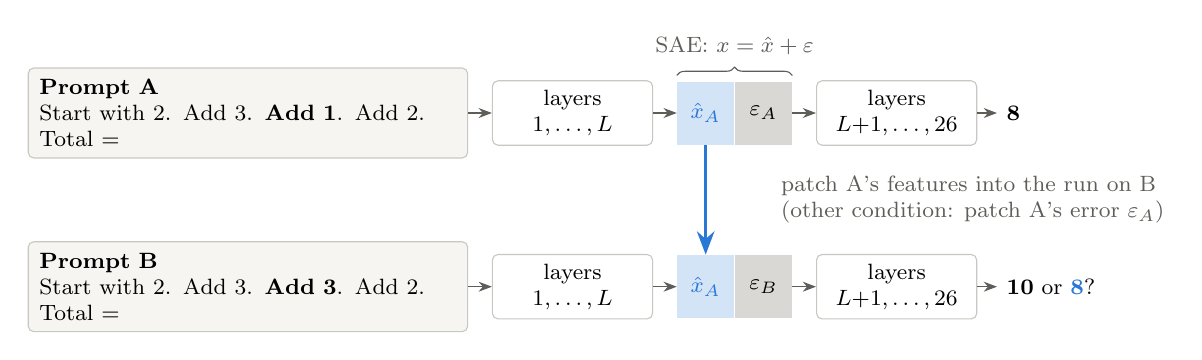
\begin{tikzpicture}[>=Stealth, font=\footnotesize,
  prompt/.style={draw=light, fill=paper, rounded corners=2pt, align=left, text width=5.3cm, inner sep=4pt},
  blk/.style={draw=light, fill=white, rounded corners=2pt, minimum height=0.8cm, align=center, text width=1.8cm},
  part/.style={minimum width=0.72cm, minimum height=0.8cm, inner sep=0pt},
  lab/.style={color=ink2}]
  \node[prompt] (pa) at (0,0) {\textbf{Prompt A}\\Start with 2. Add 3. \textbf{Add 1}. Add 2. Total~=};
  \node[blk, right=0.3cm of pa] (la) {layers\\$1,\dots,L$};
  \node[part, fill=accent!20, right=0.3cm of la] (fa) {\color{accent}$\hat{x}_A$};
  \node[part, fill=light!70, right=0pt of fa] (ea) {$\varepsilon_A$};
  \node[blk, right=0.3cm of ea] (ra) {layers\\$L{+}1,\dots,26$};
  \node[right=0.25cm of ra] (oa) {\textbf{8}};
  \node[prompt, below=1.05cm of pa] (pb) {\textbf{Prompt B}\\Start with 2. Add 3. \textbf{Add 3}. Add 2. Total~=};
  \node[blk, right=0.3cm of pb] (lb) {layers\\$1,\dots,L$};
  \node[part, fill=accent!20, right=0.3cm of lb] (fb) {\color{accent}$\hat{x}_A$};
  \node[part, fill=light!70, right=0pt of fb] (eb) {$\varepsilon_B$};
  \node[blk, right=0.3cm of eb] (rb) {layers\\$L{+}1,\dots,26$};
  \node[right=0.25cm of rb, align=left] (ob) {\textbf{10} or \textbf{\color{accent}8}?};
  \foreach \a/\b in {pa/la, la/fa, ea/ra, ra/oa, pb/lb, lb/fb, eb/rb, rb/ob} \draw[->, ink2] (\a) -- (\b);
  \draw[->, very thick, accent] (fa.south) -- (fb.north);
  \draw[decorate, decoration={brace, amplitude=3pt}, ink2] ([yshift=2pt]fa.north west) -- ([yshift=2pt]ea.north east)
    node[midway, above=4pt, lab] {SAE: $x = \hat{x} + \varepsilon$};
  \node[lab, anchor=west, align=left] at ($(ea.south)!0.5!(eb.north) + (0.1,0)$)
    {patch A's features into the run on B\\(other condition: patch A's error $\varepsilon_A$)};
\end{tikzpicture}
}
  \caption{Activation patching with an SAE. The SAE splits each activation at layer $L$ into features $\hat{x}$ and
    error $\varepsilon$. Patching A's features into the run on B and checking whether the answer moves from 10 to 8
    shows how much of the task's information the features carry; the second condition patches A's error instead.}
  \label{fig:method}
\end{figure}

\textbf{Findings} (Appendix~\ref{app:results}):
\begin{enumerate}[label=\textbf{\arabic*.}]
  \item \textbf{Features carry most of the effect.} On the three tracking tasks, patching $\hat{x}$ recovers 74--100\%
    at every layer tested (4 to 20); patching $\varepsilon$ recovers 0--13\%, except object tracking at layers 8--16
    (25--62\%), which is mostly an artefact: replacing B's error with noise of the same size, which merely erases it,
    already recovers 28--58\%. The names control loses 24--36\% at layers 18--20.
  \item \textbf{A concentrated gap.} For object tracking at layer 12, $\hat{x}$ recovers 74\% (95\% CI 73--76\%). Also
    restoring A's error along the direction in which the task's training errors vary most raises this to 88\%, about
    half of the gap; a random direction adds nothing (Figure~\ref{fig:repair}).
  \item \textbf{Task specificity.} Two same-task directions close 39--53\% of that gap; directions from other tasks
    close $-1$ to 2\%, from generic text 1\%. The running sum at layer 18 (gap 13\%) behaves alike (25--58\% vs at most
    1\%); the names gap at layer 18 is diffuse (about 32 directions to close half).
  \item \textbf{Width.} From 16k to 262k features the object-tracking gap goes 26, 20, 24, 23, 15\%, and one error
    direction still closes 51--69\% of it; wider SAEs also use more active features, so width stays open.
  \item \textbf{Pitfalls.} Patching only the last token, probing without a prompt-only baseline, and equating what a
    probe can read with what the model uses would each have misled us (Appendix~\ref{app:traps}).
\end{enumerate}

\begin{figure}[t]
  \centering
  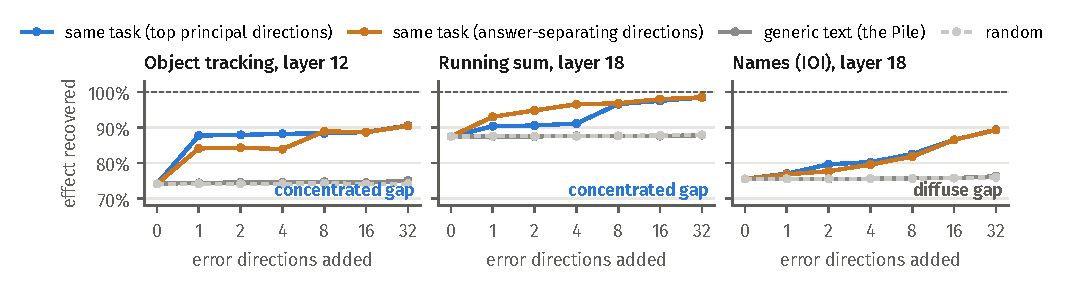
\includegraphics[width=\linewidth]{p_repair.pdf}
  \caption{Concentrated and diffuse gaps. Effect recovered when the features are combined with A's error along $N$
    directions. For object tracking and the running sum, one or two directions estimated on the same task close much of
    the gap; directions from generic text or random directions close nothing. The names gap closes only slowly.}
  \label{fig:repair}
\end{figure}

\textbf{Limitations.} One model, one SAE family, synthetic tasks, width at one layer; patching along a few directions
can create effects the model does not normally use~\citep{makelov2024subspace}, which our controls address only in part.

%==============================================================================
\section{How: plan and success criteria}

\textbf{Q1, generality.} We group tasks by the computation they need: \emph{entity binding} (objects in boxes; people
and their cities, e.g.\ ``Asha lives in Pune. Ravi lives in Delhi. Asha lives in''), \emph{counting} (longer running
sums), \emph{reference following} (variable copying) and the names control. Per task, layer and width we measure the
gap, the directions needed to close half of it, and a \term{specificity score} (share closed by same-task directions
minus the largest share from any other source). Transfer between the two binding tasks separates a template-specific
gap from a computation-specific one; SAEs with equal numbers of active features separate width from sparsity.

\textbf{Q2, mechanism.} Feng and Steinhardt~\citep{feng2024bind} found that LLaMA and Pythia models mark each entity and
its attribute with a shared ``binding ID'' vector. We will estimate these for gemma-2-2b, compare them with the
object-tracking error direction, and shift activations along it to test whether the answer moves to the other box.

\textbf{Q3, language.} The same tasks in Hindi (Devanagari), Hinglish (Latin script, with English words), Hindi in
Latin script without English words, Tamil or Bengali where the model can do them, and French as a non-Indian control.
Example: \hindi{शुरुआत \lat{2} से करें। \lat{3} जोड़ें। \lat{1} जोड़ें। \lat{2} जोड़ें। कुल
\lat{=}}{shuruaat 2 se karen. 3 joden. 1 joden. 2 joden. kul =} $\to$ 8 (design in Appendix~\ref{app:design}).

\begin{table}[htbp]
\centering\small
\caption{Success criteria, fixed in advance. All comparisons use 95\% confidence intervals; a result that meets
  neither column is reported as inconclusive.}
\label{tab:criteria}\footnotesize
\begin{tabularx}{\linewidth}{@{}l Y Y@{}}
\toprule
Question & Supported if & Not supported if \\
\midrule
Q1 & gap $\geq$ 10\%, and same-task directions close $\geq$ 30 points more than any other source; transfer
  between binding tasks $\geq$ half of own & on $\geq$ 2 new tasks with a gap, other sources close as much as same-task
  directions \\
Q2 & shifting along the direction moves $\geq$ 50\% of pairs to the other box; a random direction $\leq$ 5\% & the
  shift is no more effective than a random direction \\
Q3 & Hindi gap larger than English, with non-overlapping intervals (fidelity and transfer criteria in
  Table~\ref{tab:multi}) & Hindi gap not larger \\
\bottomrule
\end{tabularx}
\end{table}

\textbf{Deliverables:} (1) a table of gap size, type and specificity for every task, layer, width and language;
(2) the patching code, with the three pitfalls handled; (3) a result on the binding hypothesis. \textbf{Resources:} one
8\,GB GPU and the tested pilot pipeline (the main pilot runs took about 6.3 hours); risks and fallbacks are listed in
Appendix~\ref{app:design}.

%==============================================================================
\section{When: timeline}

\begin{table}[H]
\centering\small
\caption{Timeline. Each half-week ends with a checkpoint.}
\label{tab:timeline}
\begin{tabularx}{\linewidth}{@{}l Y l@{}}
\toprule
Dates & Work & Checkpoint \\
\midrule
Oct 19--26 & Pilot study, four stages (done; Appendix~\ref{app:runs}) & concentrated gap found \\
Oct 27--29 & Q2: binding vectors and the shifting test; Q1: new tasks & Q2 result \\
Oct 30--Nov 2 & Q1: matched-sparsity widths; Q3: task performance in Hindi, Hinglish & usable languages \\
Nov 3--9 & Q1: gap and specificity per task; Q3: fidelity, gap, transfer & Q1 and Q3 tables \\
Nov 10--12 & Buffer; more test pairs; robustness checks & final figures \\
Nov 13--16 & Report and final presentation & submission \\
\bottomrule
\end{tabularx}
\end{table}

{\small
\setlength{\bibsep}{1.5pt}
\bibliographystyle{compact}
\bibliography{../refs}
}

%==============================================================================
\clearpage
\appendix
% In the appendices, keep each section's floats inside that section.
\let\oldsection\section
\renewcommand{\section}{\FloatBarrier\oldsection}
\renewcommand{\thetable}{\thesection.\arabic{table}}
\renewcommand{\thefigure}{\thesection.\arabic{figure}}
\makeatletter\@addtoreset{table}{section}\@addtoreset{figure}{section}\makeatother
\begin{center}{\Large\bfseries Appendices}\\[2pt]{\color{muted}The original plan, the pilot methods and every pilot
result}\end{center}
\vspace{-2pt}
\begin{center}\small
\begin{tabular}{@{}l l@{}}
\ref{app:original} & From the original plan to the pilot tasks \\
\ref{app:methods} & Pilot methods: model and SAEs, tasks, patching, repair, probes, runs \\
\ref{app:results} & Pilot results: patching, repair, specificity, width, pitfalls, replication, verdict, caveats \\
\ref{app:design} & Design of the planned study \\
\ref{app:glossary} & Glossary \\
\end{tabular}
\end{center}

%------------------------------------------------------------------------------
\section{From the original plan to the pilot tasks}\label{app:original}

\subsection{Original hypotheses}
The project began as \emph{PRISM} (Probing Residual Information and State Manifolds), a test of a strong version of the
``dark matter'' hypothesis: that SAEs fail to represent the step-by-step state a model computes, so that this state
resides in the SAE error. It made three hypotheses, each tied to one experiment (Table~\ref{tab:hyp}).

\begin{table}[H]
\centering\small
\caption{The original hypotheses and the experiment designed to test each.}
\label{tab:hyp}
\begin{tabularx}{\linewidth}{@{}l Y Y Y@{}}
\toprule
& Hypothesis & Experiment & Prediction if true \\
\midrule
H1 & The SAE error carries the task state & Patch $\hat{x}$ or $\varepsilon$ from prompt A into the run on prompt B &
  patching $\varepsilon$ recovers more than patching $\hat{x}$ \\
H2 & The state forms a low-dimensional structure in the error & Spread of $\varepsilon$ across directions; probes for the
  state; low-dimensional projections & a probe reads the state from $\varepsilon$ better than from $\hat{x}$ and better
  than from the prompt's words \\
H3 & A few error directions repair the SAE & Features plus A's error along its top $r$ directions & a small $r$ closes
  most of the gap; random directions do not \\
\bottomrule
\end{tabularx}
\end{table}

\subsection{Original tasks and planned runs}
Three algorithmic tasks whose answer depends on a hidden running state: a sum with a remainder (modular arithmetic),
the depth of nested brackets, and the size of the graph reachable from a node, with the names task as a control. The
planned runs used layers 4--24 (every fourth), SAE widths 16k and 65k, 400 training and 200 test pairs, up to 64 error
directions and two extra direction types (top directions of $\hat{x}$; directions spanning both parts). They were
organised in tiers for a single 24\,GB GPU: a core tier (six layers $\times$ two widths $\times$ two patch positions),
a tier over all 26 layers, a width tier (16k to 524k) and an expansion tier (1000/500 pairs, a second seed, generic-text
directions).

\subsection{The overnight run of October 19 and the code checks}
The overnight run kept no usable pairs: after filtering, the three algorithmic tasks retained 10\%, 21\% and 16\% of
candidate pairs, the names control was dropped as unsolvable under that run's prompt format, and the core tier produced
no results. A code check on October 20 then found pipeline problems as well as model limits: the few-shot examples were
drawn after the training and test pairs had used up the prompt space (0 of 2 examples were added); the bracket-depth
and names tasks could not fill their test sets (0 of 1400 and 144 of 600 candidates); the zero-shot names prompt was
answered correctly only 69\% of the time; and the installed transformers library (5.x) is untested with
TransformerLens. All were fixed before the pilot: examples are now drawn first, and each task's prompt format, number
of examples and difficulty were chosen in the capability study below. The same check confirmed that our model matches
Hugging Face's implementation: the same top answer on 95\% of prompts (largest logit difference 4.7, median 0.49 in
16-bit precision), correct answers on 6 of 7 sanity prompts for both (both miss ``The capital of France is''), identical
outputs when a run resumes from a middle layer, and identical scores in batched and single runs.

\subsection{Capability study}
On October 20 we measured each task on 128 pairs per setting, with 0, 2, 4 or 8 worked examples and several difficulty
levels. A setting is usable if the model's top answer is correct on at least 60\% of prompts, at least 30\% of pairs
pass the pair filter, and the lower end of the 95\% (Wilson) interval beats the best shortcut, such as repeating the
starting number or the last number added. The three original tasks failed at every setting (Table~\ref{tab:capability});
for bracket depth, 83\% of wrong answers simply repeated the starting depth. A probe could read bracket depth from the
activations (99\%), but a probe on the prompt's tokens alone did as well (100\%), so this was not evidence of internal
state.

\begin{table}[H]
\centering\small
\caption{Capability study. Original tasks at their planned difficulty; replacement tasks at the setting used in the
  pilot runs (``kept in run'' is the share of generated pairs that passed the pilot's pair filter).}
\label{tab:capability}
\begin{tabularx}{\linewidth}{@{}l Y r r r@{}}
\toprule
Task & Setting & Top answer correct & Best shortcut & Kept in run \\
\midrule
Sum with remainder & 4 steps, best of 0--8 examples & 13\% & 21\% & -- \\
Bracket depth & 8 operations, best of 0--8 examples & 41\% & 41\% & -- \\
Graph size & 4 edges, best of 0--8 examples & 30\% & 48\% & -- \\
\midrule
Running sum & 3 steps, 8 examples & 98\% & 26\% & 62\% \\
Object tracking & 2 moves, 8 examples & 98\% & 65\% & 27\% \\
Variable copying & 1 hop, 2 examples & 22\% & 16\% & 40\% \\
Names (IOI) & 2 examples & 100\% & 17\% & 100\% \\
\bottomrule
\end{tabularx}
\end{table}

Variable copying is weak at 2 examples in the capability study (it reaches 95\% with 8), but the pilot runs used 2
examples with a stricter filter and a larger pool of candidates, which still left 300 training and 150 test pairs of
cases the model solves.

%------------------------------------------------------------------------------
\section{Pilot methods}\label{app:methods}

\subsection{Model and SAEs}\label{app:model}

\begin{table}[H]
\centering\small
\caption{Model, SAEs and their quality.}
\label{tab:model}
\begin{tabularx}{\linewidth}{@{}l Y@{}}
\toprule
Item & Value \\
\midrule
Model & gemma-2-2b: 26 layers, 2304 numbers per token, run in 16-bit (bf16) precision \\
SAEs & Gemma Scope residual-stream SAEs with a JumpReLU activation~\citep{lieberum2024gemmascope,rajamanoharan2024jumping}
  (\texttt{gemma-scope-2b-pt-res-canonical}); widths 16k, 32k, 65k, 131k and 262k \\
Fidelity (16k) & next-token performance kept on generic text: 99.1\% (layer 10), 98.7\% (12), 98.5\% (14), 98.0\%
  (18), relative to replacing the activation by its average; 3936 tokens of the Pile \\
Error size (16k) & $\|\varepsilon\|/\|x\|$ on the pilot prompts: 0.08--0.09 at layer 4, 0.12--0.18 at layers 8--16,
  0.11--0.13 at layer 20 \\
Compute & one 8\,GB laptop GPU (RTX 5060) \\
\bottomrule
\end{tabularx}
\end{table}

\subsection{Tasks}\label{app:tasks}
Each task generator produces pairs whose prompts have the same number of tokens and whose answers are single tokens;
pairs that break this are dropped and counted. Worked examples are prepended identically to both prompts. The
\term{pair filter} keeps only pairs the model handles: \emph{strict} requires the model's top answer to be correct on
both prompts and its preference for A's answer over B's to exceed 2 logits on prompt A; \emph{clean-only} requires a
correct top answer on prompt A and a change in preference of more than 2 logits between the prompts. A task is skipped
if fewer than 20 pairs survive.

\begin{table}[H]
\centering\small
\caption{Task settings in the main pilot. ``Preference'' is the mean logit difference between A's and B's answer on
  prompt A and on prompt B; chance is one over the number of possible answers.}
\label{tab:tasksettings}
\begin{tabularx}{\linewidth}{@{}l Y r l r r r@{}}
\toprule
Task & Difficulty & Examples & Filter & Kept & Preference A / B & Chance \\
\midrule
Running sum & 3 steps & 8 & strict & 62\% & 3.48 / $-$3.02 & 25\% \\
Object tracking & 3 objects, 2 moves & 8 & clean-only & 27\% & 2.77 / $-$0.15 & 18\% \\
Variable copying & 1 copy hop & 2 & strict & 40\% & 3.11 / $-$2.81 & 11\% \\
Names (IOI) & -- & 2 & strict & 100\% & 6.75 / $-$6.39 & 11\% \\
\bottomrule
\end{tabularx}
\end{table}

The running sum also uses a story form (``Anna has 5 cards. Anna gets 1 more. Anna gets 2 more. Anna gets 1 more.
Anna now has'' $\to$ 9; in B the second step becomes ``gets 1 more'' $\to$ 8). Variable copying always opens with a
distracting assignment, so that ``the first number'' is not a shortcut.

\subsection{Activation patching}\label{app:patching}
\textbf{Effect recovered} (NLDR, normalized logit-difference recovery). A \emph{logit} is the model's raw score for a
possible next token. With $D$ the logit of A's answer minus the logit of B's answer,
$\mathrm{NLDR} = (D_{\text{patched}} - D_{B})/(D_{A} - D_{B})$, averaged over test pairs: 0 means no change, 1 means
the same as patching the whole activation. Values can exceed 1. Intervals are 95\% paired bootstrap intervals
(1000 resamples).

\textbf{Conditions} (all at one layer; the subscript names the prompt each part comes from):
\begin{description}[leftmargin=1.2em, style=nextline, itemsep=1pt, font=\normalfont\itshape]
  \item[Features only, error only, full activation] $\hat{x}_A + \varepsilon_B$; $\hat{x}_B + \varepsilon_A$; and
    $x_A$, which gives 1 by construction.
  \item[Noise control] $\hat{x}_B + \eta$, with random noise $\eta$ of the same size as $\varepsilon$: it erases B's
    error without supplying A's.
  \item[Features alone] $\hat{x}_A$ with no error at all.
  \item[Error resampling] (last token only) $\hat{x}_B$ plus the error of another pair whose prompt A has the same
    answer, or a different answer; and $\hat{x}_B$ plus the average training error. If the error carried the answer,
    same-answer resampling would beat different-answer resampling.
\end{description}

\textbf{Positions.} Every result patches all tokens from the first one where A and B differ, except pitfall~1, which
patches the last token only (Figure~\ref{fig:positions}).

\begin{figure}[H]
  \centering
  % Patch positions: last token only vs every token from the first one that differs.
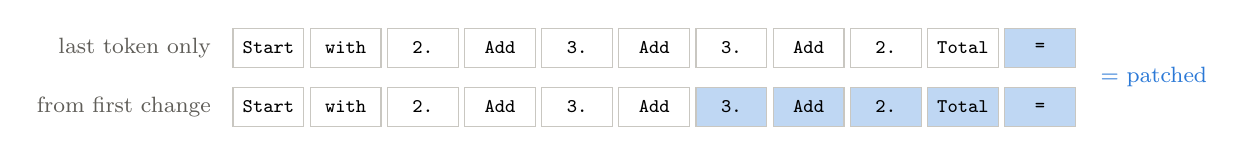
\begin{tikzpicture}[font=\footnotesize,
  tok/.style={draw=light, minimum height=0.5cm, minimum width=0.9cm, inner sep=1pt, font=\scriptsize\ttfamily},
  lab/.style={color=ink2, anchor=east}]
  \foreach \row/\y/\lbl in {1/0/last token only, 2/-0.75/from first change} {
    \node[lab] at (-0.15,\y) {\lbl};
    \foreach \t [count=\i] in {Start,with,2.,Add,3.,Add,3.,Add,2.,Total,=} {
      \pgfmathsetmacro{\hl}{(\row==1 && \i==11) || (\row==2 && \i>=7) ? 1 : 0}
      \ifdim\hl pt>0.5pt
        \node[tok, fill=accent!30, anchor=west] at ({(\i-1)*0.98},\y) {\t};
      \else
        \node[tok, fill=white, anchor=west] at ({(\i-1)*0.98},\y) {\t};
      \fi
    }
  }
  \node[color=accent, anchor=west] at (10.9,-0.375) {= patched};
\end{tikzpicture}

  \caption{Patch positions for a running-sum pair. Earlier tokens are identical in A and B, so patching from the first
    changed token onwards covers everything that differs; the last token alone may not yet hold the state.}
  \label{fig:positions}
\end{figure}

\textbf{Decision rules, fixed before the run.} H1 is judged only at layers where patching the full activation recovers
at least 0.8. A gap counts as persistent across widths if the widest SAE keeps at least 60\% of the 16k gap.

\subsection{Repair with error directions}\label{app:repair}

\begin{figure}[H]
  \centering
  % Repair: the run on B gets A's features, A's error along r chosen directions, and B's error in every other direction.
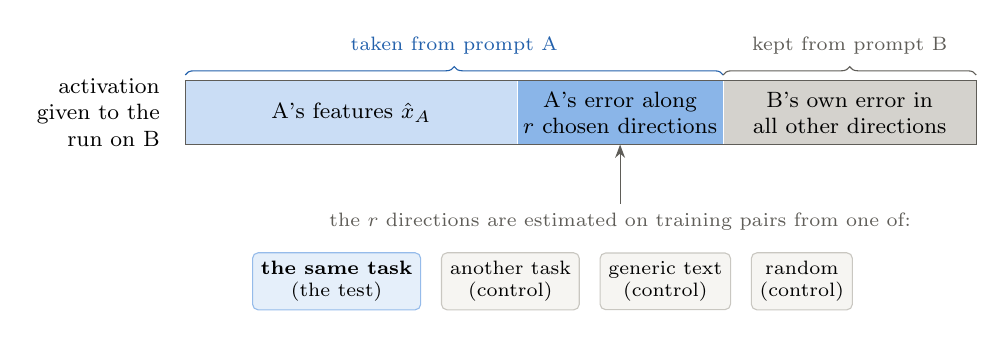
\begin{tikzpicture}[font=\footnotesize, >=Stealth,
  seg/.style={minimum height=0.8cm, inner sep=2pt, align=center},
  src/.style={draw=light, fill=paper, rounded corners=2pt, inner sep=3pt, font=\scriptsize, align=center},
  lab/.style={color=ink2, align=center, font=\scriptsize}]
  % The patched activation, drawn as one bar
  \node[seg, fill=accent!25, minimum width=4.2cm] (f) {A's features $\hat{x}_A$};
  \node[seg, fill=accent!55, minimum width=2.6cm, right=0pt of f] (r) {A's error along\\$r$ chosen directions};
  \node[seg, fill=light!80, minimum width=3.2cm, right=0pt of r] (o) {B's own error in\\all other directions};
  \draw[ink2] (f.north west) rectangle (o.south east);
  \node[left=0.2cm of f, align=right] {activation\\given to the\\run on B};
  \draw[decorate, decoration={brace, amplitude=3pt}, accent!80!black] ([yshift=2pt]f.north west) -- ([yshift=2pt]r.north east)
    node[midway, above=4pt, lab, color=accent!80!black] {taken from prompt A};
  \draw[decorate, decoration={brace, amplitude=3pt}, ink2] ([yshift=2pt]o.north west) -- ([yshift=2pt]o.north east)
    node[midway, above=4pt, lab] {kept from prompt B};
  % Where the directions come from
  \node[lab, below=0.75cm of r.south, anchor=north] (q) {the $r$ directions are estimated on training pairs from one of:};
  \node[src, below=0.15cm of q.south, xshift=-3.6cm, fill=accent!12, draw=accent!50] (s1) {\textbf{the same task}\\(the test)};
  \node[src, right=0.25cm of s1] (s2) {another task\\(control)};
  \node[src, right=0.25cm of s2] (s3) {generic text\\(control)};
  \node[src, right=0.25cm of s3] (s4) {random\\(control)};
  \draw[->, ink2] (q.north) -- (r.south);
\end{tikzpicture}

  \caption{Repair. The run on B receives A's features, A's error along $r$ chosen directions, and B's own error in all
    other directions.}
  \label{fig:repairdiag}
\end{figure}

Directions are estimated on the 300 training pairs only: \emph{top principal directions} are the directions in which the
task's training errors vary most; \emph{answer-separating directions} are the principal directions of the differences
between the average errors for each answer. Other sources: the same estimate on another task (\emph{transfer}), on
generic text (the Pile, 40--100 documents of 128 tokens), or random directions (2--3 seeds). We test $r = 0, 1, 2, 4, 8,
16, 32$ (and 64 in the audit run). The \term{share of the gap closed} is (repair $-$ features only) / gap.

\subsection{Probes}\label{app:probes}
A probe is a linear classifier trained on the training pairs to read the answer from the activation at the last token,
and scored on the test pairs. We probe $x$, $\hat{x}$, $\varepsilon$ and the SAE's feature activations (2048 columns),
report accuracy and selectivity (accuracy minus the accuracy with shuffled labels), and compare with the same probe on
the prompt's tokens alone.

\subsection{Runs, compute and failures}\label{app:runs}

\begin{figure}[H]
  \centering
  % The four pilot stages and the three main runs.
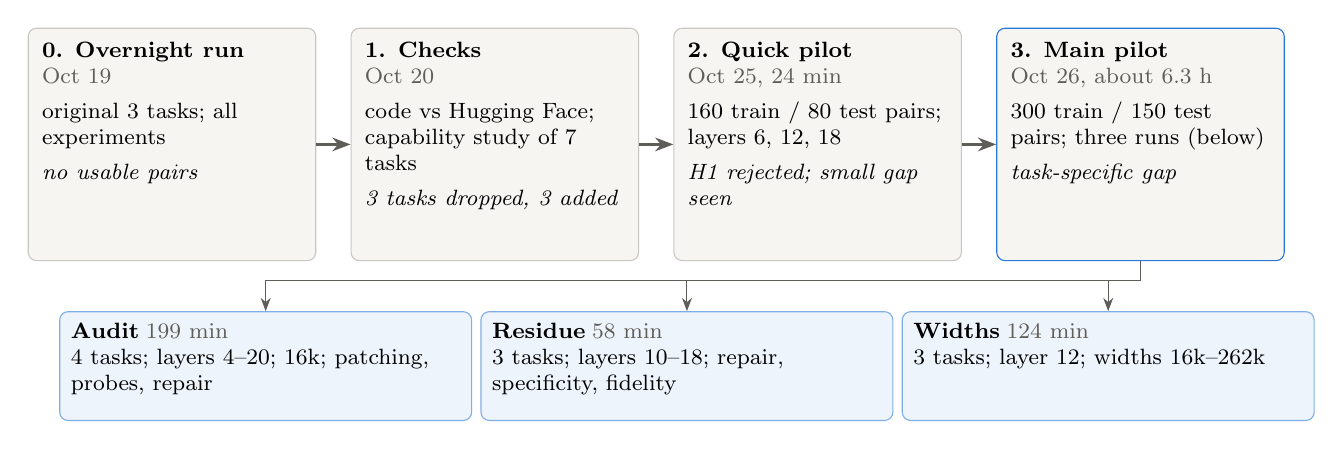
\begin{tikzpicture}[>=Stealth, font=\footnotesize,
  st/.style={draw=light, fill=paper, rounded corners=3pt, inner sep=5pt, anchor=north west},
  run/.style={draw=accent!60, fill=accent!8, rounded corners=3pt, inner sep=4pt, anchor=north west}]
  \newcommand{\stage}[4]{\parbox[t][2.6cm][t]{3.3cm}{\raggedright\textbf{#1}\\{\color{ink2}#2}\\[3pt]#3\\[3pt]\textit{#4}}}
  \node[st] (a) at (0,0) {\stage{0. Overnight run}{Oct 19}{original 3 tasks; all experiments}{no usable pairs}};
  \node[st] (b) at (4.1,0) {\stage{1. Checks}{Oct 20}{code vs Hugging Face; capability study of 7 tasks}{3 tasks dropped, 3 added}};
  \node[st] (c) at (8.2,0) {\stage{2. Quick pilot}{Oct 25, 24 min}{160 train / 80 test pairs; layers 6, 12, 18}{H1 rejected; small gap seen}};
  \node[st, draw=accent] (d) at (12.3,0) {\stage{3. Main pilot}{Oct 26, about 6.3 h}{300 train / 150 test pairs; three runs (below)}{task-specific gap}};
  \foreach \x/\y in {a/b, b/c, c/d} \draw[->, thick, ink2] (\x.east) -- (\y.west);
  \newcommand{\runbox}[3]{\parbox[t][1.1cm][t]{4.95cm}{\raggedright\textbf{#1}\;{\color{ink2}#2}\\#3}}
  \node[run] (r1) at (0.4,-3.6) {\runbox{Audit}{199 min}{4 tasks; layers 4--20; 16k; patching, probes, repair}};
  \node[run] (r2) at (5.75,-3.6) {\runbox{Residue}{58 min}{3 tasks; layers 10--18; repair, specificity, fidelity}};
  \node[run] (r3) at (11.1,-3.6) {\runbox{Widths}{124 min}{3 tasks; layer 12; widths 16k--262k}};
  \draw[->, ink2] (d.south) |- ++(0,-0.25) -| (r1.north);
  \draw[->, ink2] (d.south) |- ++(0,-0.25) -| (r2.north);
  \draw[->, ink2] (d.south) -- ++(0,-0.25) -| (r3.north);
\end{tikzpicture}

  \caption{The four pilot stages. The main pilot consisted of three runs on one 8\,GB GPU.}
  \label{fig:pipeline}
\end{figure}

\begin{table}[H]
\centering\small
\caption{Run inventory (all with 16k SAEs unless stated).}
\label{tab:runs}
\begin{tabularx}{\linewidth}{@{}l Y Y r@{}}
\toprule
Run & Tasks and layers & Experiments & Time \\
\midrule
Quick pilot & 4 tasks; layers 6, 12, 18; 160/80 pairs & patching (both positions, controls); repair at 12, 18;
  300 bootstrap resamples & 24 min \\
Audit & 4 tasks; layers 4, 8, 12, 16, 20 & patching (both positions, controls); probes at 8--20; repair up to 64
  directions & 199 min \\
Residue & 3 tasks (no variable copying); layers 10, 12, 14, 18 & patching; repair with generic-text and transfer
  directions; fidelity & 58 min \\
Widths & 3 tasks; layer 12; widths 16k--262k & patching; repair; fidelity & 124 min \\
\bottomrule
\end{tabularx}
\end{table}

\textbf{Failures.} In the residue run, estimating repair directions at layer 10 failed (the singular value
decomposition did not converge), so there are no repair results at layer 10. In the widths run, repair for the names
task at 65k ran out of GPU memory, so Table~\ref{tab:width} has no repair entry for that case.

%------------------------------------------------------------------------------
\section{Pilot results}\label{app:results}

\subsection{Features versus error, by layer}

\begin{figure}[H]
  \centering
  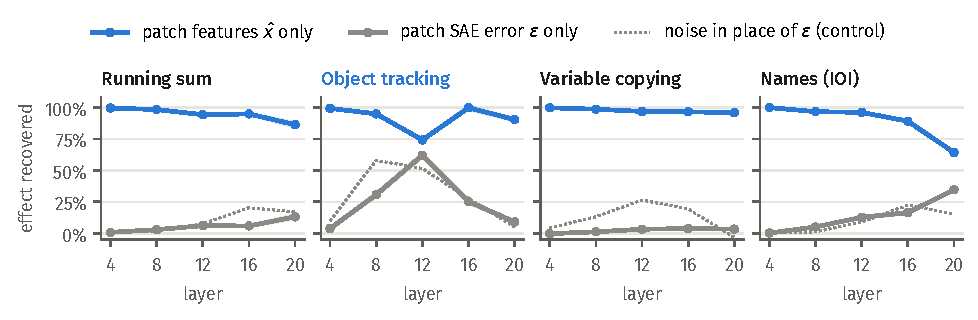
\includegraphics[width=\linewidth]{p_split.pdf}
  \caption{The features carry most of the effect at every layer; the error alone carries little. Shaded bands are 95\%
    intervals. Object tracking's error curve at layers 8--16 follows the noise control, so most of it comes from
    erasing B's error rather than from A's error.}
  \label{fig:split}
\end{figure}

\begin{table}[H]
\centering\small
\caption{Effect recovered (\%) by patching the features / the error, per layer.}
\label{tab:split}
\begin{tabular}{@{}l c c c c c@{}}
\toprule
Task & Layer 4 & Layer 8 & Layer 12 & Layer 16 & Layer 20 \\
\midrule
Running sum & 99 / 1 & 98 / 3 & 94 / 6 & 95 / 6 & 86 / 13 \\
Object tracking & 99 / 4 & 95 / 31 & 74 / 62 & 100 / 25 & 90 / 9 \\
Variable copying & 100 / 0 & 99 / 1 & 97 / 3 & 96 / 4 & 96 / 3 \\
Names (IOI) & 100 / 0 & 97 / 5 & 96 / 13 & 89 / 16 & 64 / 35 \\
\bottomrule
\end{tabular}
\end{table}

Further controls at layer 12 (effect recovered, \%): the noise control gives 7, 51, 26 and 9 for the four tasks in the
order of Table~\ref{tab:split}; features alone give 102, 109, 77 and 97. For object tracking at the last token,
same-answer error resampling gives 28, different-answer resampling 26 and the average error 13, against 28 for patching
A's own error: the error's effect does not depend on which answer it came from, which again argues against H1.

\subsection{Repair}

\begin{table}[H]
\centering\small
\caption{Repair for every case with a gap of at least 5\% (layers 8--20). Share of the gap closed (\%) by one and two
  directions (top principal / answer-separating), by two generic-text and two random directions, and the number of
  directions needed to close half of the gap. Variable copying has no gap of 5\% or more.}
\label{tab:repair}
\begin{tabular}{@{}l c c c c c c c@{}}
\toprule
Task & Layer & Gap & 1 direction & 2 directions & Generic (2) & Random (2) & For half \\
\midrule
Running sum & 12 & 6 & $-$2 / 9 & $-$4 / 18 & 0 & 1 & $>$32 / $>$32 \\
 & 14 & 6 & $-$1 / 14 & $-$5 / 22 & $-$1 & 2 & $>$32 / $>$32 \\
 & 16 & 5 & $-$4 / 36 & 6 / 46 & -- & $-$1 & 32 / 4 \\
 & 18 & 13 & 23 / 44 & 25 / \textbf{58} & 0 & 1 & 8 / \textbf{2} \\
 & 20 & 14 & 19 / 14 & 23 / 43 & -- & 0 & 8 / 4 \\
\midrule
Object tracking & 8 & 5 & $-$16 / $-$8 & $-$26 / 0 & -- & 0 & $>$32 / $>$32 \\
 & 12 & 26 & \textbf{52} / 38 & 53 / 39 & 1 & 0 & \textbf{1} / 8 \\
 & 18 & 14 & $-$2 / 26 & 18 / 36 & 2 & 1 & 16 / 4 \\
 & 20 & 10 & $-$32 / 29 & $-$6 / 47 & -- & $-$2 & 16 / 4 \\
\midrule
Names (IOI) & 14 & 10 & 1 / 2 & 1 / 2 & 1 & 0 & $>$32 / $>$32 \\
 & 16 & 11 & $-$1 / $-$3 & $-$13 / $-$6 & -- & 0 & $>$32 / $>$32 \\
 & 18 & 24 & 6 / 5 & 17 / 9 & 0 & 0 & 32 / 32 \\
 & 20 & 36 & 10 / 9 & 19 / 15 & -- & 0 & 16 / 16 \\
\bottomrule
\end{tabular}
\end{table}

Only two cases are concentrated in the sense of the hypothesis (one or two directions close half the gap): object
tracking at layer 12 and the running sum at layer 18. The other gaps need 4 to more than 32 directions, and small gaps
give noisy, sometimes negative, shares. Generic-text directions were tested only in the residue run (layers 12, 14 and
18; ``--'' elsewhere).

\subsection{Task specificity}

\begin{table}[H]
\centering\small
\caption{Share of the gap closed (\%) by two directions from each source.}
\label{tab:spec}
\begin{tabular}{@{}l l c@{}}
\toprule
Task (gap) & Source & Share closed \\
\midrule
Object tracking, layer 12 (26\%) & same task: top principal / answer-separating & 53 / 39 \\
 & other task: names / running sum & 2 / $-$1 \\
 & generic text / random & 1 / 0 \\
\midrule
Running sum, layer 18 (13\%) & same task: top principal / answer-separating & 25 / 58 \\
 & other task: object tracking / names & 1 / 0 \\
 & generic text / random & 0 / 1 \\
\bottomrule
\end{tabular}
\end{table}

\subsection{Width}

\begin{figure}[H]
  \centering
  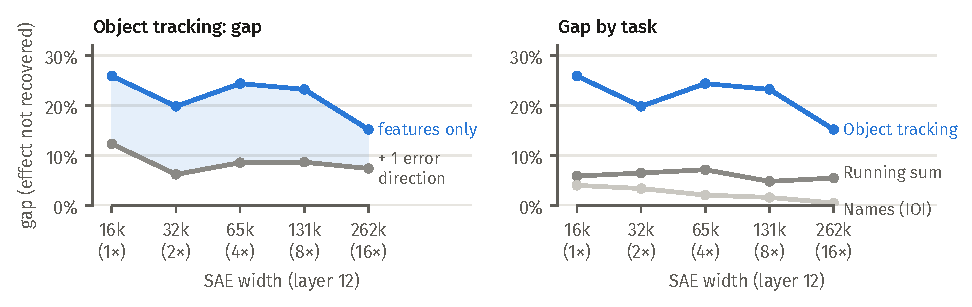
\includegraphics[width=\linewidth]{p_width.pdf}
  \caption{Wider SAEs at layer 12. Left: the object-tracking gap with the features only and with one error direction
    added; the shaded band is what that direction closes. Right: the gap for three tasks.}
  \label{fig:width}
\end{figure}

\begin{table}[H]
\centering\small
\caption{Width sweep at layer 12 (\%). ``+1 error'' and ``+1 random'' add one top principal or random direction;
  ``active'' is the mean number of features switched on per token.}
\label{tab:width}
\begin{tabular}{@{}l l c c c c c@{}}
\toprule
Task & Width & Features only [95\% CI] & Gap & +1 error & +1 random & Active \\
\midrule
Object tracking & 16k & 74 [73, 76] & 26 & 88 & 74 & 78 \\
 & 32k & 80 [79, 82] & 20 & 94 & 80 & 75 \\
 & 65k & 76 [74, 77] & 24 & 91 & 76 & 76 \\
 & 131k & 77 [75, 78] & 23 & 91 & 77 & 131 \\
 & 262k & 85 [84, 86] & 15 & 93 & 85 & 124 \\
\midrule
Running sum & 16k & 94 [93, 95] & 6 & 94 & 94 & 80 \\
 & 32k & 94 [92, 95] & 6 & 94 & 94 & 80 \\
 & 65k & 93 [91, 94] & 7 & 93 & 93 & 75 \\
 & 131k & 95 [94, 96] & 5 & 95 & 95 & 131 \\
 & 262k & 95 [93, 96] & 5 & 94 & 95 & 129 \\
\midrule
Names (IOI) & 16k & 96 [95, 97] & 4 & 96 & 96 & 89 \\
 & 32k & 97 [96, 98] & 3 & 97 & 97 & 82 \\
 & 65k & 98 [97, 99] & 2 & -- & -- & 82 \\
 & 131k & 98 [98, 99] & 2 & 98 & 98 & 138 \\
 & 262k & 100 [99, 100] & 0 & 100 & 100 & 139 \\
\bottomrule
\end{tabular}
\end{table}

The 262k SAE keeps 15.2\% of the 25.9\% object-tracking gap (59\%), just under the 60\% persistence rule
(Appendix~\ref{app:patching}). The 131k and 262k SAEs also switch on more features per token than the narrower ones, so
part of the drop may come from sparsity rather than width.

\subsection{Three pitfalls}\label{app:traps}

\textbf{Pitfall 1: patching only the last token.} In early and middle layers the state still sits on earlier tokens,
so patching only the last token recovers little even with the whole activation (Table~\ref{tab:positions}); patching
from the first changed token recovers 100\% at every task and layer~\citep{zhang2024towards}.

\begin{table}[H]
\centering\small
\caption{Effect recovered (\%) when the whole activation is patched at the last token only.}
\label{tab:positions}
\begin{tabular}{@{}l c c c c c@{}}
\toprule
Task & Layer 4 & Layer 8 & Layer 12 & Layer 16 & Layer 20 \\
\midrule
Running sum & 0 & 0 & 3 & 58 & 94 \\
Object tracking & 1 & 4 & 47 & 77 & 85 \\
Variable copying & 0 & 0 & 0 & 5 & 55 \\
Names (IOI) & 0 & 0 & 0 & 60 & 81 \\
\bottomrule
\end{tabular}
\end{table}

\textbf{Pitfall 2: the prompt gives the answer away.} A probe on the prompt's tokens alone scores 100\% on variable
copying and names (Table~\ref{tab:probes}), so a high probe score there says nothing about the model's internal
state~\citep{hewitt2019designing}. \textbf{Pitfall 3: readable is not used.} For object tracking and names, probes read
the answer far better from $\varepsilon$ than from $\hat{x}$ (84 vs 48\%; 97 vs 20\%), yet patching that token recovers
at most 47\%: the model is not yet using the information at that position.

\begin{table}[H]
\centering\small
\caption{Probe accuracy at the last token, layer 12 (\%), and the effect of patching that token.}
\label{tab:probes}
\begin{tabular}{@{}l c c c c c c@{}}
\toprule
Task & Probe on $x$ & On $\varepsilon$ & On $\hat{x}$ & Prompt tokens only & Chance & Last-token patch \\
\midrule
Running sum & 57 & 53 & 42 & 45 & 25 & 3 \\
Object tracking & 91 & 84 & 48 & 33 & 18 & 47 \\
Variable copying & 98 & 95 & 39 & 100 & 11 & 0 \\
Names (IOI) & 100 & 97 & 20 & 100 & 11 & 0 \\
\bottomrule
\end{tabular}
\end{table}

\subsection{Replication: quick pilot versus main pilot}

\begin{table}[H]
\centering\small
\caption{The quick pilot (160/80 pairs) and the main pilot (300/150 pairs) agree.}
\label{tab:replication}
\begin{tabular}{@{}l c c@{}}
\toprule
Quantity & Quick pilot & Main pilot \\
\midrule
Object tracking, layer 12: features only / error only / noise control & 75 / 61 / 50 & 74 / 62 / 51 \\
Object tracking, layer 12: share of gap closed by one direction & 51 & 52 \\
Running sum, layer 18: gap & 12 & 13 \\
Names, layer 18: gap; share closed by 32 directions & 24; 55 & 24; 56 \\
\bottomrule
\end{tabular}
\end{table}

\subsection{Verdict on the original hypotheses}

\begin{table}[H]
\centering\small
\caption{What the pilot says about each original hypothesis.}
\label{tab:verdict}
\begin{tabularx}{\linewidth}{@{}l Y@{}}
\toprule
Hypothesis & Verdict \\
\midrule
H1 (error carries the state) & \textbf{Rejected} for every task: $\hat{x}$ recovers more than $\varepsilon$ at every
  layer, and the error's effect does not depend on which answer it came from. \\
H2 (low-dimensional structure in the error) & \textbf{Not supported as stated}: the answer can be read from
  $\varepsilon$ but is not used there, and for two tasks the prompt's words alone give it away. \\
H3 (a few directions repair) & \textbf{Supported, narrowly}: one direction closes about half of object tracking's gap
  at layer 12, and two close 58\% of the running sum's at layer 18; the directions are task-specific. This became the
  project's hypothesis. \\
\bottomrule
\end{tabularx}
\end{table}

\subsection{Caveats}\label{app:caveats}
\begin{itemize}
  \item One model (gemma-2-2b), one SAE family (Gemma Scope) and synthetic tasks; width was tested at layer 12 only.
  \item Object tracking is the hardest task for the model: only 27\% of generated pairs passed its filter, so its test
    pairs are the most heavily selected and may over-represent easier cases.
  \item The names control's late-layer loss (24--36\% at layers 18--20) is spread over many directions: part of the
    late-layer loss is a general SAE weakness rather than a task-specific gap.
  \item Width and sparsity are confounded in the Gemma Scope family (Table~\ref{tab:width}).
  \item The binding explanation is a hypothesis, and the multilingual work is a plan with no results yet.
\end{itemize}

%------------------------------------------------------------------------------
\section{Design of the planned study}\label{app:design}

\begin{figure}[H]
  \centering
  % Planned study: per-language flow and the task-by-language grid.
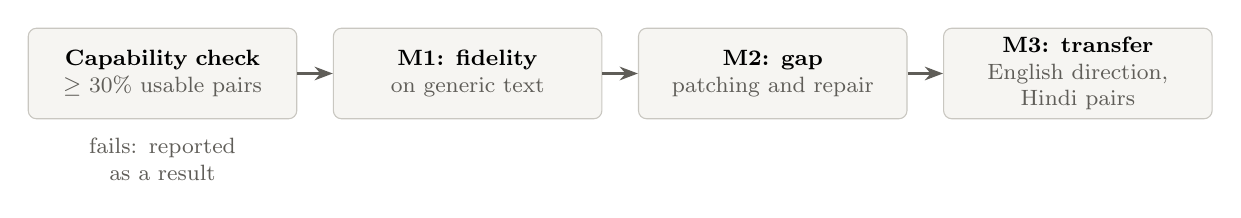
\begin{tikzpicture}[>=Stealth, font=\footnotesize,
  st/.style={draw=light, fill=paper, rounded corners=3pt, align=center, text width=3.2cm, minimum height=1.15cm, inner sep=3pt}]
  \node[st] (g) at (0,0) {\textbf{Capability check}\\{\color{ink2}$\geq$ 30\% usable pairs}};
  \node[st, right=0.45cm of g] (m1) {\textbf{M1: fidelity}\\{\color{ink2}on generic text}};
  \node[st, right=0.45cm of m1] (m2) {\textbf{M2: gap}\\{\color{ink2}patching and repair}};
  \node[st, right=0.45cm of m2] (m3) {\textbf{M3: transfer}\\{\color{ink2}English direction,\\Hindi pairs}};
  \foreach \a/\b in {g/m1, m1/m2, m2/m3} \draw[->, thick, ink2] (\a) -- (\b);
  \node[color=ink2, below=0.12cm of g, text width=3.1cm, align=center] {fails: reported as a result};
\end{tikzpicture}

  \caption{Steps for each language. A language passes on only if the model can do the tasks in it.}
  \label{fig:design}
\end{figure}

\begin{table}[H]
\centering\small
\caption{Multilingual measures and criteria (95\% intervals; otherwise inconclusive).}
\label{tab:multi}
\begin{tabularx}{\linewidth}{@{}l Y Y Y@{}}
\toprule
ID & Measure & Supported if & Not supported if \\
\midrule
M1 & fidelity on generic text, per language & Hindi $\geq$ 3 points below English & within 1 point of English \\
M2 & gap and specificity on the tasks & Hindi gap larger, non-overlapping intervals & Hindi gap not larger \\
M3 & English direction applied to Hindi pairs & closes $\geq$ half as much as Hindi's own direction & closes under a
  quarter as much \\
\bottomrule
\end{tabularx}
\end{table}

\textbf{Languages.} English (baseline); Hindi in Devanagari (the best-resourced Indian language, most likely to work);
the same Hindi in Latin script without English words, and Hinglish (Latin script, mixed with English words), which
together separate the effect of script from that of vocabulary; Tamil or Bengali if the model can do the tasks; French
as a high-resource non-Indian control. Q2 (binding) is run in English only.

\textbf{Templates.} The answer must be the last token. Arithmetic templates can end with ``='' as in English; templates
that need a verb at the end in Hindi use a question followed by ``answer:''. Examples (single-token answers are checked
against the tokenizer before use):
\begin{itemize}
  \item Object tracking (Hindi): \hindi{सिक्का डिब्बे \lat{B} में है। चाबी डिब्बे \lat{E} में है। चाबी डिब्बे \lat{C} में
    चली जाती है। चाबी किस डिब्बे में है? \mbox{डिब्बा~$\to$~\lat{C}}}{sikka dibbe B mein hai. chaabi dibbe E mein hai. chaabi dibbe C
    mein chali jaati hai. chaabi kis dibbe mein hai? dibba $\to$ C}
  \item \raggedright Names (Hinglish): \prompt{Jab Rahul aur Priya market gaye, Priya ne ek book di. Book kisko mili?
    Answer:} $\to$ Rahul
  \item Variable copying is code-like and identical in every language: a language-neutral control.
\end{itemize}
\textbf{Constraints.} Prompts A and B need the same number of tokens and a one-token answer; many Hindi names split
into several tokens, so names are chosen from single-token ones (the pipeline already drops and counts pairs that break
this rule). \textbf{Data.} Fidelity per language uses generic text from IndicCorp~v2~\citep{doddapaneni2023towards}
and FineWeb2~\citep{penedo2025fineweb2}.

\textbf{Risks and fallbacks.}
\begin{itemize}
  \item Binding vectors may not be estimable for gemma-2-2b; Q2 then keeps only the shifting test.
  \item The model may not do the tasks in Tamil or Bengali; we report this and keep Hindi and Hinglish.
  \item Names that split into several tokens are replaced by letters or digits as answers.
  \item Width results at one layer may not generalise; Q1 repeats them at a second layer if time allows.
\end{itemize}

%------------------------------------------------------------------------------
\section{Glossary}\label{app:glossary}

\begin{table}[H]
\centering\small
\caption{Terms used in this proposal.}
\label{tab:glossary}
\begin{tabularx}{\linewidth}{@{}l Y@{}}
\toprule
Term & Meaning \\
\midrule
Token & a word or word piece; the unit the model reads \\
Layer & one of gemma-2-2b's 26 processing stages \\
Activation $x$ & the model's internal vector for one token at one layer (2304 numbers; also ``residual stream'') \\
Sparse autoencoder (SAE) & a tool that rewrites an activation as a few active, interpretable features \\
Features $\hat{x}$ & the SAE's reconstruction of $x$ from its active features \\
SAE error $\varepsilon$ & $x - \hat{x}$: what the SAE does not explain (``dark matter''; informally, the leftovers) \\
Width & how many features an SAE can choose from (16k = 16{,}384, up to 262k) \\
Active features & the number of features switched on for one token (also L0) \\
Reconstruction fidelity & share of next-token performance kept when $\hat{x}$ replaces $x$, relative to replacing $x$ by
  its average (cross-entropy loss recovered) \\
Prompts A and B & two prompts that differ in one step, so the right answer differs (also ``clean'' and ``corrupt'') \\
Activation patching & running the model on B while replacing part of its activation with A's at one layer \\
Logit & the model's raw score for a possible next token \\
Effect recovered (NLDR) & how far patching moves the model's preference from B's answer to A's, from 0 to 1 \\
Gap & the effect the features fail to carry: one minus the effect recovered by patching the features only \\
Direction & a fixed vector in the 2304-dimensional activation space \\
Top principal directions & the directions in which a set of errors varies most \\
Answer-separating directions & directions that best separate the average errors for different answers \\
Specificity score & share of the gap closed by same-task directions minus the largest share from any other source \\
Probe & a simple linear classifier trained to read a value, such as the box, from an activation \\
Binding & how a model links an entity to its attribute, such as an object to its box \\
IOI & ``indirect object identification'', the names task~\citep{wang2023interpretability} \\
Generic text & ordinary text from the Pile, used for fidelity and for generic-text directions \\
Hinglish & Hindi written in Latin script and mixed with English words \\
95\% CI & bootstrap confidence interval: the range the result would likely fall in on new test pairs \\
\bottomrule
\end{tabularx}
\end{table}

\end{document}
